\documentclass[aspectratio=169]{beamer}
\usepackage{xcolor}
\usepackage{hyperref}
\usepackage{graphicx}
\usepackage{minted}
\usepackage{bookmark}
\usepackage{amsmath}
\usepackage{amssymb}
\usepackage{amsfonts} % loads maths fonts
\usepackage{geometry}
\usepackage{esint}
\usepackage{systeme}
\usepackage{tikz}
\usepackage{pgf}
\usepackage{booktabs}
\usepackage{subcaption}
\usepackage{enumerate}
\usepackage{relsize}
\usepackage{multirow}
\usepackage{multicol}
\usepackage{ulem}
\usepackage{systeme}
\usepackage{longtable}
\usepackage{newverbs}
\usepackage{xurl}
\usepackage{listings}
\usepackage{float}
\usemintedstyle{autumn}
\setminted{
    breaklines,
    fontsize=\footnotesize,
    tabsize=4,
    xleftmargin=2em
}
\setmintedinline{
	fontsize=\footnotesize
}

\newmintinline[LC]{latex}{}
\newmintinline[LCS]{latex}{fontsize=\scriptsize}
\newminted[LCL]{latex}{}
\newcommand{\LCX}[1]{$#1$ & \LC|#1|}
\newverbcommand{\LCXV}%
{\VerbatimOut{\jobname.tmp}}%
{\endVerbatimOut%
1 & 1}
\DeclareMathOperator{\Mr}{M_{\mathbb{R}}}
\floatstyle{ruled}
\newfloat{program}{thp}{lop}
\floatname{program}{Program}

\newenvironment{warning}{\begin{center}\begin{minipage}{\textwidth}\large \bf \color{red}}{\end{minipage}\end{center}}
\newenvironment{latexexample}{\begin{example}}{\end{example}}
\newenvironment{command}{\begin{block}{Command}}{\end{block}}
\newcommand{\samplebegin}[1]{\structure{\textbackslash begin}\{#1\}}
\newcommand{\sampleend}[1]{\structure{\textbackslash end}\{#1\}}
\newcommand{\samplecommand}[1]{\alert{\textbackslash #1}}
\newcommand{\samplecolorbox}[1]{\fcolorbox{black}{#1}{\color{#1}{\tiny{\phantom{0000}}}} \small{#1}}
\newcommand{\sampletext}[2]{\samplecommand{#1} - {#2{Sample Text}}}
\newcommand{\sampleaccent}[3]{\samplecommand{#1}\{#3\}\quad #2{#3}}
\newcommand{\samplesymbol}[2]{\samplecommand{#1}\quad #2}
\newcommand{\urllink}[1]{\href{#1}{\beamergotobutton{Link}}}
\newcommand{\packagename}[1]{\structure{\texttt{#1}}}

\newenvironment{latexexampleframe}
{\VerbatimOut{\jobname.tmp}}
{\endVerbatimOut

\begin{frame}
\begin{example}
\inputminted{latex}{./\jobname.tmp}
\end{example}
\end{frame}

\begin{frame}
\input{./\jobname.tmp}
\end{frame}
}

\newenvironment{latexexamplesplit}
{\VerbatimOut{\jobname.tmp}}
{\endVerbatimOut

\begin{example}
\begin{minipage}{0.48\textwidth}
~
\inputminted{latex}{./\jobname.tmp}
\end{minipage}
\hfill
\begin{minipage}{0.48\textwidth}
\input{./\jobname.tmp}
\end{minipage}
\end{example}
}


\setbeamertemplate{navigation symbols}{}
\setbeamertemplate{section in toc}[sections numbered]

\hypersetup{colorlinks=true,linkcolor=purple,filecolor=magenta,urlcolor=purple}
\AtBeginSection[]{
    \begin{frame}{Table of Contents}
        \small
        \begin{multicols}{2}
        \tableofcontents[currentsection]
        \end{multicols}
    \end{frame}
}

\urlstyle{same}

\title{Introduction to \LaTeX\  from a Practical Perspective}
\author{\hyperlink{https://github.com/TechJI-2023/latex_wksp}{Z. Zhou}, \hyperlink{https://github.com/evs000}{M. Huang}, \hyperlink{https://github.com/fakefred}{fkfd}, \hyperlink{https://github.com/Hydraallen}{R. Wang}}
\institute{TechJI}
\date{\today}
\begin{document}

\begin{frame}
    \titlepage
    \begin{figure}
        \centering
        \caption*{Wechat Group}
        \includegraphics[width=2.5cm]{./qrcode.jpg}
    \end{figure}
\end{frame}

\begin{frame}{Agenda}
    \begin{itemize}
        \item General Introduction to \LaTeX \hspace*{\fill} \textit{by} Z.~Zhou
        \item Introduction to \packagename{Tikz} \hspace*{\fill} \textit{by} Z.~Zhou
        \item Beamer \hspace*{\fill} \textit{by} Y.~Yin
        \item Introduction to \packagename{Bibtex} \hspace*{\fill} \textit{by} M.~Huang
    \end{itemize}
\end{frame}

\section{Introduction to \LaTeX}

\subsection{What is \LaTeX}

\begin{frame}{What is \LaTeX}
    \begin{block}{From Wikipedia, the free encyclopedia\footnotemark[1]}
        \LaTeX\ (lah-tekh, lah-tek or lay-tek, a shortening of Lamport \TeX) is a document preparation system. When writing, the writer uses plain text in markup tagging conventions to define the general structure of a document (such as \structure{article}, \structure{book}, and \structure{letter}), to stylize text throughout a document (such as \textbf{bold} and \textit{italic}), and to add citations\footnotemark[1] and cross-references. \medskip

        \pause

        A \TeX\ distribution such as \TeX Live or Mik\TeX\ is used to produce an output file (such as PDF or DVI) suitable for printing or digital distribution. \medskip

        \pause

        Within the typesetting system, its name is stylized as \LaTeX.
    \end{block}

    \footnotetext[1]{\LaTeX\ - \url{https://en.wikipedia.org/wiki/LaTeX}}

\end{frame}

\begin{frame}{Comparison with other Typesetting Systems}
    \begin{itemize}[<+->]
        \item Advantages over MS Word
        \begin{itemize}[<+->]
            \item Plain text file, easy version control
            \item Wide range of packages and templates
            \item Open-source
        \end{itemize}
        \item Advantages over \hyperlink{https://typst.app/}{typst}
        \begin{itemize}[<+->]
            \item Larger community and packages
        \end{itemize}
        \item Drawbacks
        \begin{itemize}[<+->]
            \item Long compile time
            \item Too many symbols and commands to remember
            \item Bad, unclear, hard-to-understand error messages
        \end{itemize}
    \end{itemize}    
\end{frame}

\begin{frame}{A brief History of \TeX\ and \LaTeX}
    Donald Kunuth from Stanford University is the specialist in programming art. In year 1977, he had just received his first samples from the new typesetting system of the publisher's, and its quality was so far below that of the first edition of Volume 2 that he couldn't stand it. Kunuth decided to implement a mathematical composition system by himself (since he is a computer scientist). He figured that this would take about 6 months (Ultimately, it took nearly 10 years). The system is named as \TeX, of both the meaning of Greek letters $\tau\epsilon\chi$, and ``technical ''. \medskip

    \pause

    \LaTeX\ was created in 1983 by Leslie Lamport, when he was working at SRI. He needed to write \TeX\ macros for his own use, and thought with a little extra effort he could make a general package usable by others. Then \LaTeX\  developed rapidly and now there are thousands of packages written in \TeX\ macros available for direct usage.

\end{frame}

\subsection{Distributions and IDEs}

\begin{frame}{Write \LaTeX\ on Overleaf (Online)}
    Another alternative choice is to write \LaTeX\ online with the technology of \href{https://www.overleaf.com/}{Overleaf}.
    It's free for personal usage and supports share editing which is very useful in group work.
    A SJTU hosted Overleaf instance can be found \href{https://latex.sjtu.edu.cn/}{here}.
    \begin{figure}
        \centering
        \includegraphics[width=0.6\linewidth]{../intro/overleaf.png}
        \caption{Layout of the Overleaf Online \LaTeX\ Editor.}
    \end{figure}
\end{frame}


\begin{frame}{Installation of \LaTeX}
    Though there are some other distributions of \LaTeX (like Mik\TeX), \TeX Live is recommended in this workshop (or you can use Overleaf instead).

    We recommend beginners to use VS Code as IDE to edit \LaTeX\  files.
    See Hydraallen's \href{https://github.com/Hydraallen/Latex-vscode}{latex-vscode} for installing \TeX Live and \LaTeX\  extension for VS Code.
\end{frame}

\subsection{Documentation}

\begin{frame}[fragile]{Documentation of \LaTeX}

    If you've installed a full version of \TeX Live (as strongly recommended), the full \LaTeX\ documentation is already on your computer. \medskip

    \pause

    Open the command line and input the command

    \begin{minted}{shell}
texdoc <docname>
    \end{minted}

    \pause

    You can also use the online version on \urllink{https://www.latex-project.org/help/documentation/} \medskip

    \pause

    For example, you can use the following types for the \structure{docname}
    \begin{description}
        \item[tex] 		about \structure{\TeX}
        \item[article] 	about documentclass \packagename{article}
        \item[beamer] 	about documentclass \packagename{beamer} (used to create slides)
        \item[pgf]		about packages \packagename{tikz} and \packagename{pgf} (used to draw graphs)
    \end{description}

    \pause

    \smallskip
    Try to \alert{texdoc} about all new things and then you'll be an expert in \LaTeX.
\end{frame}

\subsection*{Starter Pack}

\begin{frame}{Inexperienced \LaTeX\  User Starter Pack}
    \begin{figure}[h]
        \centering
        \includegraphics[width=0.8\textwidth]{../intro/latex_user.png}
    \end{figure}
    \tiny{Frederick Yin, Inexperienced LaTeX User Starter Pack}
\end{frame}

\begin{frame}{Inexperienced \LaTeX\  User Starter Pack 2.0}
    \begin{figure}[h]
        \centering
        \includegraphics[width=0.8\textwidth]{../intro/latex_user_2.png}
    \end{figure}
    \tiny{Frederick Yin, Inexperienced \LaTeX\  Users Starter Pack v2.0}
\end{frame}

\section{Basics}

\subsection{Global Structure}

\begin{frame}[fragile]{Global Structure}

While in many cases you don't write \LaTeX documents from scratch (eg. using templates), you should still know the basic structure of a \LaTeX document (can help you fix bugs!).

Every input file must contain the commands:

\begin{command}
\begin{minted}{latex}
\documentclass{...}

\begin{document}
...
\end{document}
\end{minted}
\end{command}
The area between \LC|\documentclass{...}| and \LC|\begin{document}| is called the \textit{preamble}. It normally contains commands that affect the entire document.

You would put your text where the dots are between \LC|\begin{document}| and \LC|\end{document}|.
        
\end{frame}

\begin{frame}[fragile]{Document Class}
    You need to set the layout standard for your document. This is done by specifying a \textit{document class}.
    \begin{command}
        \begin{minted}{latex}
\documentclass[options]{class}
        \end{minted}
    \end{command}
    \pause
    For example, you can use \LC|\documentclass[11pt,twoside,a4paper]{article}| to initialize an article with a base font size of 11 points, and to produce a layout suitable for double sided printing on A4 paper.

    \pause

    You can see a list of document classes in \href{https://ctan.org/topic/class}{CTAN Class} and options in \href{https://en.wikibooks.org/wiki/LaTeX/Document_Structure}{Document Structure}.
\end{frame}

\begin{frame}[fragile]{Packages}
    In the preamble area, you can load extra packages.

    \begin{command}
        \begin{minted}{latex}
\usepackage[options]{package}
% or
\usepackage{package1,package2}
        \end{minted}
    \end{command}
    \pause
    For example, if you want to have more detailed settings for the layout of your document, you can use the \textit{geometry} package.

    \pause
    
    A simple example would be:

    \begin{command}
        \begin{minted}{latex}
\usepackage[a4paper,left=2.5cm,right=2.5cm,top=2cm,bottom=2cm]{geometry}
        \end{minted}
    \end{command}

    This would set a new layout for A4 paper with 2.5cm margins on the left and right, and 2cm margins on the top and bottom of each page.

    \pause

    See \href{https://www.overleaf.com/learn/latex/Page_size_and_margins}{Page size and margins} for more details on page layout.
\end{frame}

\begin{frame}[fragile]{Top Matter}
    At the beginning of most documents there will be information about the document itself, such as the title and date, and also information about the authors, such as name, address, email etc.

    All of this type of information within \LaTeX is collectively referred to as \textit{top matter}.

    \pause

    \begin{command}
        \begin{minted}{latex}
...
\begin{document}
\title{LaTeX Document Sample}
\author{Your name}
\date{\today}
\maketitle
\tableofcontents
\end{document}
        \end{minted}
    \end{command}

    \pause
    You need to use \LC|\maketitle| to generate the final title. If you omit the \LC|\date| command, \LaTeX will use today's date based on the typographic rules.

    \pause
    \LC|\tableofcontents| will generate a table of contents based on the sections of your document.
\end{frame}

\begin{frame}[fragile]{Document body}
    In order for the table of contents to display something it is necessary to add different levels of headings.

    \begin{command}
        \begin{minted}{latex}
...
\begin{document}
...

\section{sec1}
\subsection{sec1.1}
\subsubsection{sec1.1.1}

\section{sec2}
\subsection{sec2.1}
\subsubsection{sec2.1.1}
\end{document}
        \end{minted}
    \end{command}
    \pause
    To hide the number, add * like \LC|\section*{sec3}|, but be aware that it will not be shown in the table of contents.
\end{frame}

\subsection{Modular Documents}

\begin{frame}[fragile]{Multiple files}
    \LaTeX allows you to split the content of your document into separate files. This is particularly useful if you want to create a book or a large report.

    \pause

    \begin{command}
        \begin{minted}{latex}
\documentclass{article}
\begin{document}
\input{titlepage}
\input{introduction}
\input{section1}
\input{section2}
\end{document}
        \end{minted}
    \end{command}

    This file will input the contents of the files \textit{titlepage.tex}, \textit{introduction.tex}, \textit{section1.tex} and \textit{section2.tex} in that order. What it does is effectively copy and paste the contents of the files into the document in the order that they are listed.

\end{frame}

\begin{frame}[fragile]{Graphics Path}
    When you want to include a figure from file, you normally write \LC|\includegraphics{figures/filename}|. However, if you have a lot of figures, you may want to put them in a separate folder. In this case, you can use \LC|\graphicspath| to specify the path to the folder.

    \pause

    Write the following commands in preamble:
    
    \begin{command}
        \begin{minted}{latex}
\graphicspath{{figures/}}
% or many folders
\graphicspath{{subdir1/}{subdir2/}{subdir3/}...{subdirn/}}
        \end{minted}
    \end{command}
    After that, you can simply use \LC|\includegraphics{filename}| to include the figure.
\end{frame}

\section{Text}

\subsection{Special Characters}

\begin{frame}
    \frametitle{Special Characters}
    Some special symbols can't be directly used since they are reserved by \LaTeX:
    \begin{center}
        \begin{tabular}{llllll}
            \LC|\#|               & \#                                                                                                                            \\
            \samplesymbol{\#}{\#} & \samplesymbol{\$}{\$} & \samplesymbol{\%}{\%} & \samplesymbol{\&}{\&} & \samplesymbol{\~{}}{\~{}} & \samplesymbol{\`{}}{\`{}} \\
            \samplesymbol{\{}{\{} & \samplesymbol{\}}{\}} & \samplesymbol{\_}{\_} &
            \multicolumn{2}{l}{\samplesymbol{backslash}{$\backslash$}}
        \end{tabular}
    \end{center}

    \pause

    Many \LaTeX\ starters are confused with how to correctly print quotes, hyphens and dots.\\
    \pause
    \`{} prints a left single quote, ' prints a right single quote.\\
    \pause
    \`{}\`{} prints a left double quote, '' prints a right double quote.\\
    \pause
    one hyphen (-) print like - \\
    \pause
    two hyphens ({-}{-}) print like -- \\
    \pause
    three hyphens ({-}{-}{-}) print like ---\\
    \pause
    \samplecommand{dots} prints the dots with a correct format (\dots) instead of directly use three dots (...)
\end{frame}

\begin{frame}{Warning}
    \begin{warning}
        Do NOT use {\tt "} and {\tt '} to print quotes.
    \end{warning}
\end{frame}

\begin{frame}
    \frametitle{Deal with unfamiliar symbols}
    Sometimes you may want to deal with symbols you have never seen. In this case, you may refer to \url{http://detexify.kirelabs.org/classify.html} to find out how to output the character.
\end{frame}

\subsection{Fonts}

\begin{frame}
    \frametitle{Basic commands about fonts}
    First, lets start with some commands that transform font types
    \pause
    \begin{itemize}
        \item \sampletext{bf}{\bf}
        \item \sampletext{it}{\it}
        \item \sampletext{rm}{\rm}
        \item \sampletext{sc}{\sc}
        \item \sampletext{sf}{\sf}
        \item \sampletext{sl}{\sl}
        \item \sampletext{tt}{\tt}
    \end{itemize}
    \pause
    Note that the commands that transform font types influence the text in the whole scope (\structure{\{...\}}) until another font type is specified. For example, how to use the first command \samplecommand{bf} is shown below\\[0.5em]
    \{\samplecommand{bf} Sample Text\}
\end{frame}

\begin{frame}[fragile]
    Sometimes we don't want to transform  all the font types, instead, we can only change the font type of some specified text.
    \pause
    \begin{example}
        \begin{minted}{latex}
\textbf{Sample text}
		\end{minted}
    \end{example}
    \pause
    There are more options for fonts.
    \begin{itemize}
        \item \sampletext{textit}{\textit}
        \item \sampletext{textsc}{\textsc}
        \item \sampletext{texttt}{\texttt}
    \end{itemize}
    \pause
    However, in a math environment (will be introduced later), some other commands should be used
    \begin{itemize}
        \item \samplecommand{mathbf} - $\mathbf{Sample\ Text}$
        \item \samplecommand{mathsf} - $\mathsf{Sample\ Text}$
    \end{itemize}
    \pause
    Note that the math environment doesn't include all of the font types on the previous page. More information about font types can be found \href{http://www.cnblogs.com/make217/p/6123532.html}{here}.
\end{frame}

\begin{frame}
    Font size can also be easily modified
    \begin{itemize}
        \item \sampletext{tiny}{\tiny}
        \item \sampletext{scriptsize}{\scriptsize}
        \item \sampletext{footnotesize}{\footnotesize}
        \item \sampletext{small}{\small}
        \item \sampletext{normalsize}{\normalsize}
        \item \sampletext{large}{\large}
        \item \sampletext{Large}{\Large}
        \item \sampletext{LARGE}{\LARGE}
        \item \sampletext{huge}{\huge}
        \item \sampletext{Huge}{\Huge}
    \end{itemize}
\end{frame}

\begin{frame}[fragile]
    \frametitle{Build a colorful document}
    Changing the color is similar to changing font types. \medskip

    If you want to transform to a color (like transforming to bold with \LC{\bf}), you can use \LC{\color{name}}. \smallskip

    Similarly, you can use \LC{\textcolor{name}} like \LC{\textbf}.\smallskip

    The background color of the whole page can be set using \LC{\pagecolor{name}}.\medskip

    \pause

    There are some defined color \structure{name} in the \structure{xcolor} package.\medskip

    \begin{tabular}{lllll}
        \samplecolorbox{black}  & \samplecolorbox{gray}     & \samplecolorbox{olive}   & \samplecolorbox{teal}  & \samplecolorbox{blue}      \\
        \samplecolorbox{green}  & \samplecolorbox{orange}   & \samplecolorbox{violet}  & \samplecolorbox{brown} & \samplecolorbox{lightgray} \\
        \samplecolorbox{pink}   & \samplecolorbox{white}    & \samplecolorbox{cyan}    & \samplecolorbox{lime}  & \samplecolorbox{purple}    \\
        \samplecolorbox{yellow} & \samplecolorbox{darkgray} & \samplecolorbox{magenta} & \samplecolorbox{red}                                \\
    \end{tabular}
    \medskip

    You can find more information in the documentation of \structure{xcolor} (\alert{texdoc} \structure{xcolor})
\end{frame}

\subsection{Underline}

\begin{frame}[fragile]
    \frametitle{Ulem package}
    If you want to add some lines on the text, use the \structure{ulem} package.
    \begin{command}
        \begin{minted}{latex}
\usepackage{ulem}
\uline{Sample Text}
		\end{minted}
    \end{command}
    \pause
    There are different kinds of lines supported:
    \begin{itemize}
        \item \sampletext{uline}{\uline}
        \item \sampletext{uuline}{\uuline}
        \item \sampletext{uwave}{\uwave}
        \item \sampletext{sout}{\sout}
        \item \sampletext{xout}{\xout}
        \item \sampletext{dashuline}{\dashuline}
        \item \sampletext{dotuline}{\dotuline}
    \end{itemize}
\end{frame}

\subsection{Enumeration}
\begin{frame}[fragile]
    \frametitle{Enumerate}
    When you need to enumerate some items as a list, you may use the \structure{enumerate} package.
    \begin{command}
        \begin{minted}{latex}
\usepackage{enumerate}
\begin{enumerate}[style]
\item % ...
\item % ...
\item % ...
\end{enumerate}
		\end{minted}
    \end{command}
    \pause
    This will generate a normal list with the serial numbers in the specified \structure{style}, which could be the following (as example)
    \begin{itemize}
        \item \alert{1} - 1, 2, 3, 4, ...
        \item \alert{(i)} - (i), (ii), (iii), (iv), ...
        \item \alert{[1.]} - [1.], [2.], [3.], [4.], ...
    \end{itemize}
\end{frame}

\begin{frame}[fragile]
    \frametitle{Itemize}
    If you want to generate an unordered list, use \structure{itemize} instead of \structure{enumerate}.
    \begin{command}
        \begin{minted}{latex}
\begin{itemize}
\item[style] % ...
\item[style] % ...
\item[style] % ...
\end{itemize}
		\end{minted}
    \end{command}
    \pause
    In this case, \structure{style} must be added after each item, which is different from that in \structure{enumerate}, and the symbol displayed in the beginning of each item will be exactly same as the \structure{style}. If \structure{style} is not added, a default style will be used.
\end{frame}

\subsection{Alignment}

\begin{frame}[fragile]
    \frametitle{Alignment}
    If you want to align a paragraph of text, use these three environments for left/center/right align.
    \begin{command}
        \begin{minted}{latex}
\begin{flushleft/center/flushright}
% ...
\end{flushleft/center/flushright}
			\end{minted}
    \end{command}
    \pause
    However, if only a single line needs to be aligned, use these three commands.
    \begin{command}
        \begin{minted}{latex}
\leftline{text}
\centerline{text}
\rightline{text}
		\end{minted}
    \end{command}
\end{frame}

\subsection{Spaces, lines and pages}

\begin{frame}
    \frametitle{Spaces may be confusing}
    There are defined command of spaces in different width and usages.
    \begin{itemize}[<+->]
        \item \textvisiblespace\ - the basic space in \LaTeX\. Note that any number of spaces or tabs is equal to one space, and the space after a command is ignored. If you want to add an extra space, use \alert{\textbackslash\textvisiblespace\ } which makes a 1/3\,em space (1 em is approximately the width of an \structure{M} in the current font)
        \item \~{} - If two words can't be separated on two lines, you can tell \LaTeX\ about it using a tie (\~{}), such as Prof.\~{}Hamade (Prof.~Hamade).
        \item  \samplecommand{,} - makes a 1/6\,em space, commonly used before units (notice the space before em on this page)
        \item  \samplecommand{;} - makes a 2/7\,em space
        \item  \samplecommand{quad} - makes a 1\,em space
        \item  \samplecommand{qquad} - makes a 2\,em space
        \item  \samplecommand{phantom}\{\structure{text}\} - makes actually the space of \structure{text}, but \structure{text} will be invisible.
    \end{itemize}
\end{frame}

\begin{frame}
    \frametitle{Separate contents into lines and pages}
    Here are some basic commands about lines and pages in \LaTeX,  you will use them everywhere.
    \pause
    \begin{itemize}[<+->]
        \item \samplecommand{newline} - begin a new line
        \item \alert{\textbackslash\textbackslash} - begin a new line (not recommended\footnotemark[1])
        \item \samplecommand{par} - begin a new paragraph (a new line with indent)
        \item \samplecommand{newpage} - begin a new page
        \item \alert{\%} - begin a line comment
    \end{itemize}
    \footnotetext[1]{According to Manuel Charlemagne, \alert{\textbackslash\textbackslash} should only be used for a force break (where \samplecommand{newline} doesn't work).}
\end{frame}

\begin{frame}{Warning}
    \begin{warning}
        Never use \alert{\textbackslash\textbackslash} to create a new line in the text, it will lead to unexpected side effects.
    \end{warning}
  \end{frame}

\begin{frame}[fragile]
    \frametitle{Spacing}
    When trying to separate two paragraphs by a certain space, many new learners of \LaTeX\ may use multiple empty lines and linebreaks, which is a very dirty fix and is not so accurate. Actually, \LaTeX\ provides a precise spacing mechanism.
    \begin{command}
        \LC{\vspace{space}}\\
        \LC{\vspace*{space}}
    \end{command}
    \pause
    When trying to show the next paragraph or sentence precisely at the bottom of the current page, we can use
    \begin{command}
        \LC{\vfill}
    \end{command}
    between the contents of two paragraphs to separate them.
\end{frame}

\begin{frame}[fragile]
    \frametitle{Predefined skipping}

    More often\footnotemark[1], we don't need to think about the skipping space, we can use the predefined skipping commands to achieve a small, medium or big skip. They are actually particular cases of \LC{\vspace}

    \begin{command}
        \LC{\smallskip}\smallskip

        \LC{\medskip}\medskip

        \LC{\bigskip}\bigskip
    \end{command}

    \pause
    You may note that the effects are these skipping commands have been already shown above.
    \footnotetext[1]{According to Manuel Charlemagne, you should always use these skipping commands if possible instead of using \alert{\textbackslash\textbackslash} (as in many online tutorials).}
\end{frame}

\begin{frame}
    \frametitle{Spacing units}
    The \structure{space} can be anything representing a size, such as \structure{1cm}, \structure{2em} and \structure{10pt}. In \LaTeX, spacing units can be
    \begin{itemize}
        \item \structure{cm}
        \item \structure{mm}
        \item \structure{in} - inch, 1 inch = 2.54 cm
        \item \structure{pt} - 72 pt = 1 inch, the smallest unit in \LaTeX
        \item \structure{em} - 1em equals to the width of letter M
        \item \structure{ex} - 1ex equals to the width of letter x
        \item \LC{\linewidth} - the width of current line in the container
        \item \LC{\pagewidth} - the width of the page
        \item \LC{\pageheight} - the height of the page
        \item \LC{\textwidth} - the normal width of text on the page
        \item \LC{\textheight} - the normal height of text on the page
    \end{itemize}
\end{frame}

\subsection{Minipage and Multicolumn}

\begin{frame}[fragile]
    \frametitle{Minipage}
    \structure{minipage} is a very useful environment for dividing pages into a grid.
    \begin{example}
        \begin{multicols}{2}
            \inputminted{latex}{../text/minipage.tex}
        \end{multicols}
    \end{example}
\end{frame}

\begin{frame}
    The code above generate six minipages in a grid of 3 columns $\times$ 2 rows. Don't try to add up the width of minipages in a line for more than about \LC{0.98\linewidth} (since a minipage have a small margin on each side), or the last minipage may be on a new line. \\[0.5em]
    For each minipage, it can be seem as an independent \LaTeX\ document, where text, formulas, graphics, tables and etc. can be inserted, and most importantly, they won't affect each other. What's more, you can even use minipages in a minipage to form a multi-level nesting. \\
\end{frame}

\begin{frame}{Example}
    \begin{minipage}{0.32\linewidth}
  Part A
\end{minipage}
\hfill % Fill horizontal space
\begin{minipage}{0.32\linewidth}
  Part B
\end{minipage}
\hfill % Fill horizontal space
\begin{minipage}{0.32\linewidth}
  Part C
\end{minipage}
\vfill % Fill vertical space
\begin{minipage}{0.32\linewidth}
  Part D
\end{minipage}
\hfill % Fill horizontal space
\begin{minipage}{0.32\linewidth}
  Part E
\end{minipage}
\hfill % Fill horizontal space
\begin{minipage}{0.32\linewidth}
  Part F
\end{minipage}

\end{frame}

\begin{frame}[fragile]
    \frametitle{The multicol package}
    When typesetting contents with small line width and many lines (for example, source code), the \structure{multicol} package is recommended.
    \begin{command}
        \begin{minted}{latex}
\usepackage{multicol}
\begin{multicols}{cols}
    % contents on column one
    \breakcolumn % break the current column here
    % contents on column two
\end{multicols}
		\end{minted}
    \end{command}
    Here \structure{cols} is the number of columns, it must be specified. If \LC{\breakcolumn} is not used, the \structure{multicol} package will automatically balance the length of each column.
\end{frame}

\section{Use Maths in \LaTeX}

\subsection{Math Expressions}

\begin{frame}[fragile]{Introduction}
Basic equations in \LaTeX\ can be easily ``programmed'', for example: 
\begin{latexexample}
The well known Pythagorean theorem \(x^2 + y^2 = z^2\) was 
proved to be invalid for other exponents. 
Meaning the next equation has no integer solutions:

\[ x^n + y^n = z^n \]
\end{latexexample}
\end{frame}

\begin{frame}[fragile]{Subscripts and Superscripts}
The use of superscripts and subscripts is very common in mathematical expressions involving exponents, indexes, and in some special operators. \footnote[1]{Some of this part is ported from the tutorial of Overleaf: \urllink{https://www.overleaf.com/learn/latex/Subscripts_and_superscripts}}

\begin{latexexamplesplit}
\[ a_1^2 + a_2^2 = a_3^2 \]
\end{latexexamplesplit}

\pause

Note that here we use \LC|\[| and \LC|\]| to typeset a mathematical expression.
You may see many people using a pair of \LC|$$| instead. It is a plain-\TeX\ command, and is nowadays heavily deprecated. See this discussion \urllink{https://tex.stackexchange.com/questions/503/why-is-preferable-to} on Stack Exchange for more information. 

\end{frame}

\begin{frame}[fragile]

If the expression contains long superscripts or subscripts, these need to be collected in braces, as \LaTeX normally applies the mathematical commands \LC{^} and \LC{_} only to the following character:

\pause

\begin{latexexamplesplit}
\[ x^{2 \alpha} - 1 = y_{ij} + y_{ij}  \]
\[ (a^n)^{r+s} = a^{nr+ns}  \]
\[ x^abc, \quad x_abc, \quad x^abc_abc \]
\[ x^{abc}, \quad x_{abc}, \quad x^{abc}_{abc} \]
\end{latexexamplesplit}

\end{frame}

\begin{frame}[fragile]{Brackets and Parentheses}
Parentheses and brackets are very common in mathematical formulas. You can easily control the size and style of brackets in \LaTeX. \footnote[1]{Some of this part is ported from the tutorial of Overleaf: \urllink{https://www.overleaf.com/learn/latex/Brackets_and_Parentheses}} \medskip

Here's how to type some common math braces and parentheses in \LaTeX: \medskip

\begin{center}
\begin{tabular}{ ccc }
Type & \LaTeX & Code \\\hline
Parentheses; round brackets	 & \LCX{(x+y)} \\
Brackets; square brackets &	 \LCX{[x+y]} \\
Braces; curly brackets	& \LCX{\{x+y\}} \\
Angle brackets	& \LCX{\langle x+y \rangle} \\
Pipes; vertical bars & \LCX{|x+y|} \\
Double pipes & \LCX{\|x+y\|} \\
Floor brackets & \LCX{\lfloor x+y \rfloor} \\
Ceil brackets & \LCX{\lceil x+y \rceil} \\
\end{tabular}
\end{center}

\end{frame}

\begin{frame}[fragile]
The size of brackets and parentheses can be manually set, or they can be resized dynamically in your document, as shown in the next example:

\begin{latexexamplesplit}
\[ F = G \left( \frac{m_1 m_2}{r^2} \right) \]
\end{latexexamplesplit}

\pause

Notice that to insert the parentheses or brackets, the \LC{\left} and \LC{\right} commands are used. Even if you are using only one bracket, both commands are mandatory, you can use invisible brackets \LC{\left.} or \LC{\right.} for this.

\begin{latexexamplesplit}
\[ \int_a^b x^2 {\sf d} x = \left. \frac{1}{3}x^3 \right|_a^b \]
\end{latexexamplesplit}

\end{frame}

\begin{frame}[fragile]
Sometimes you may want to control the sizes of the brackets yourselves, which is called manually sized brackets. The commands listed are designed for thus purpose. \medskip

\begin{center}
\begin{tabular}{ ccc }
Size & \LaTeX & Code \\[2pt] \hline
big	 & \LCX{\big( \big)} \\[5pt]
Big &	 \LCX{\Big[ \Big]} \\[5pt]
bigg	& \LCX{\bigg\{ \bigg\}} \\[5pt]
Bigg	& \LCX{\Bigg| \Bigg|} \\
\end{tabular}
\end{center}
\end{frame}

\begin{frame}[fragile]{Mathematical Modes}

\LaTeX\ allows two writing modes for mathematical expressions: the \structure{inline} mode and the \structure{display} mode. The first one is used to write formulas that are part of a text. The second one is used to write expressions that are not part of a text or paragraph, and are therefore put on separate lines. \medskip

\pause

To put your equations in \structure{inline} mode use \LC|\(| and \LC|\)|, \LC|$| and \LC|$| or \LC|\begin{math} | and \LC|\end{math}|. They all work and the choice is a matter of taste.

\pause

\begin{latexexample}
In physics, the mass-energy equivalence is stated 
by the equation $E=mc^2$, discovered in 1905 by Albert Einstein.
\end{latexexample}

\pause

The \structure{display} mode is usually used with mathematical environments together, which will be discussed in the next subsection.

\end{frame}

\begin{frame}[fragile]{Numbering of Equations}
The \structure{display} mode has two versions: \structure{numbered} and \structure{unnumbered}.

\begin{latexexample}
The mass-energy equivalence is described by the famous equation
\[E=mc^2\]
discovered in 1905 by Albert Einstein. 
In natural units ($c$ = 1), the formula expresses the identity
\begin{equation}
E=m
\end{equation}
\end{latexexample}
\end{frame}

\subsection{Math Environments}


\begin{frame}[fragile]{The \packagename{equation} Environment}
	An \packagename{equation} environment contains a set of maths equations
	\begin{command}
		\begin{minted}{latex}
\begin{equation*}
% ...
\end{equation*}
		\end{minted}
	\end{command}
	\begin{example}
		\begin{equation*}
      x = y + z
    \end{equation*}
	\end{example}
  \pause
	If a star(\structure{*}) is added, the sequence number of the equation won't be displayed (this feature is from the \packagename{amsmath} package, and should behave very similar as directly using \LC|\[| and \LC|\]|). Note that the environment name in the \LC{\begin} and \LC{\end} statements must be the same (both or neither have a \structure{*} here).
\end{frame}

\begin{frame}[fragile]
	
	In math environments, unlike in plain text, normal spaces will not lead to visible spaces in output. Only  \LC|\|\packagename{\textvisiblespace} or \LC{\quad,\qquad} etc. will create spaces between words. \medskip
	
	\LC{\partial} prints the symbol \structure{$\partial$}, \LC{\frac{...}{...}} makes a \structure{fraction}. \medskip
	
	\LC{\left(} and \LC{\right(} make \structure{braces} that fit the equation's height.	
\end{frame}

\begin{frame}[fragile]{The \packagename{split} Environment (inline)}

In order to deal with extremely long equations or equation with multiple lines, we can use the \packagename{split} environment. It is an \structure{inline} environment being used in other maths environments.
\begin{latexexamplesplit}
\begin{equation}
  \begin{split}
    F &= 1+2+3+4+5 \\
      &= 15
  \end{split}
\end{equation}
\end{latexexamplesplit}

\pause

\LC{&} is used to align the equal marks, and \LC{\\} is used to split the equation into two lines. Only one equation number will be generated in an \packagename{equation} environment. \medskip

\pause

The \packagename{split} environment is designed to serve as the entire body of an equation, or an entire line of an \packagename{align} or \packagename{gather} environment. There cannot be any printed material before or after it within the same enclosing structure. 

\end{frame}

\begin{frame}[fragile]{The \packagename{aligned} Environment (inline)}
For linear equation systems, the \packagename{aligned} environment can be used, which is similar to the \packagename{split} environment above. It is also an \structure{inline} environment, which can be used in \structure{inline} mode such as \LC|$$|! Here \packagename{split} doesn't work because \LC|\left| and \LC|\right| is an enclosing structure. See this discussion \urllink{https://tex.stackexchange.com/questions/187938/whats-the-difference-between-split-and-aligned} for more information.

\begin{latexexamplesplit}
Equations:
$
  \left\lbrace\begin{aligned}
    x+y &= 1 \\ x-y &= 1
  \end{aligned}\right.
  \Longrightarrow
  \left\lbrace\begin{aligned}
    x &= 1 \\ y &= 0
  \end{aligned}\right.
$
\end{latexexamplesplit}

Actually things can also be easier with packages like \packagename{systeme}, which will be demonstrated later.
\end{frame}

\begin{frame}[fragile]{The \packagename{align} Environment}

An \packagename{align} environment can be used to simply the \packagename{split} or \packagename{aligned} in the  \packagename{equation} environment. But it numbers the equation on each line.

\begin{latexexamplesplit}
\begin{align}
  F &= 1+2+3+4+5 \\
    &= 15
\end{align}
\end{latexexamplesplit}

Use \packagename{align*} so that there will be no number(s).

\begin{latexexamplesplit}
\begin{align*}
  a+b & \Leftrightarrow b+a \\
  (a+b)+c & \Leftrightarrow a+(b+c)
\end{align*}
\end{latexexamplesplit}

\end{frame}

\begin{frame}[fragile]

The ampersand character \LC{&} determines where the equations align. The odd columns are right-aligned, and the even ones are left-aligned, so you can use \LC{&&} if you want to make two neighbor column aligned to the same direction.

\setlength{\belowdisplayskip}{-10pt}
\begin{latexexample}
\begin{align*}
  \text{(right)} & \text{(left)} && \text{(left)} & \text{(right)} 
  &&  \text{(right)} & \text{(left)} \\
  x     &=y     &&  w   &=z        &&  a&=b+c \\
  2x    &=-y    &&  3w  &=z/2      &&  a&=b \\
  -4+5x &=2+y   &&  w+2 &=-1+w     &&  ab&=cb
\end{align*}
\end{latexexample}

\end{frame}


\begin{frame}[fragile]{The \packagename{cases} Environment (inline)}

The linear system of equations can also be typeset simply with the \packagename{cases} environment. It is less flexible than an \packagename{aligned} environment, eg., there can only be one \LC{&} on each row. Another minor difference is that the horizontal space before  \LC{&} is larger than other similar environments.

\begin{latexexamplesplit}
\begin{equation}
  \left\lbrace\begin{aligned}
    x+y &= 1 \\ 
    x-y &= 1
  \end{aligned}\right.
\end{equation}

\begin{equation}
  \begin{cases} 
    x+y &= 1 \\ 
    x-y &= 1
  \end{cases}
\end{equation}
\end{latexexamplesplit}

\end{frame}


\begin{frame}[fragile]{The \packagename{gather} Environment}

If you just need to display a set of consecutive equations, centered and with no alignment whatsoever, use the \packagename{gather} environment. The asterisk trick to set/unset the numbering of equations also works here.

\begin{latexexamplesplit}
\begin{gather} 
  2x - 5y =  8 \\ 
  3x^2 + 9y =  3a + c
\end{gather}
\end{latexexamplesplit}

\end{frame}

\begin{frame}[fragile]{The \packagename{gathered} Environment (inline) }

There is also an \structure{inline} version of \packagename{gather}, called \packagename{gathered}. The relationship of them is similar to \packagename{align} and \packagename{aligned}.

\begin{latexexamplesplit}
\begin{equation} 
  \begin{gathered} 
    2x - 5y =  8 \\ 
    3x^2 + 9y =  3a + c
  \end{gathered}
\end{equation}
\end{latexexamplesplit}

\end{frame}


\begin{frame}[fragile]{The \packagename{multline} Environment}
For equations longer than a line use the \packagename{multline} environment. Insert a double backslash to set a point for the equation to be broken. The first part will be aligned to the left and the second part will be displayed in the next line and aligned to the right.

\begin{latexexample}
\begin{multline}
  p(x) = 3x^6 + 14x^5y + 590x^4y^2 + 19x^3y^3 \\ 
         - 12x^2y^4 - 12xy^5 + 2y^6 - a^3b^3
\end{multline}
\end{latexexample}

The equation number will be in the last line, use \packagename{multline*} for no numbering.

\end{frame}

\begin{frame}[fragile]

For equations equal or longer then three lines,

\begin{latexexample}
\begin{multline*}
  a+b+c=1 \\ 
  b+c=2 \\
  c+d=1 \\
  d=3
\end{multline*}
\end{latexexample}

Here, the first column is left-aligned, the last column is right-aligned and the others ones are center-aligned. 

\end{frame}

\subsection{Spacing in Math Mode}

\begin{frame}[fragile]{Horizontal Spacing}
Horizontal spacing in maths mode is useful in several situations, let's see an example: \footnote[1]{Some of this part is ported from the tutorial of Overleaf: \urllink{https://www.overleaf.com/learn/latex/Spacing_in_math_mode}} \medskip

\begin{latexexample}
Assume we have the next sets
\[
S = \{ z \in \mathbb{C}\, |\, |z| < 1 \} \quad 
\textrm{and} \quad S_2=\partial{S}
\]
\end{latexexample}

As you see in this example, a mathematical text can be explicitly spaced by means of some special commands.

\end{frame}

\begin{frame}[fragile]
The spacing depends on the command you insert, the example below contains a complete list of spaces and how they look like.

\begin{latexexamplesplit}
\begin{align*}
f(x) =& x^2\! +3x\! +2 \\
f(x) =& x^2+3x+2 \\
f(x) =& x^2\, +3x\, +2 \\
f(x) =& x^2\: +3x\: +2 \\
f(x) =& x^2\; +3x\; +2 \\
f(x) =& x^2\ +3x\ +2 \\
f(x) =& x^2\quad +3x\quad +2 \\
f(x) =& x^2\qquad +3x\qquad +2
\end{align*}
\end{latexexamplesplit}

\end{frame}

\begin{frame}[fragile]{Vertical Spacing}
    When the space between \structure{display} maths and the main body paragraph is considered larger than expectation, is there any way to modify the line spacing? \medskip
    
    In default style of \structure{display} mode is like

\begin{latexexample}
your body paragraph is supposed to be typed here
\begin{equation}
  a \times b = c 
\end{equation}
your body paragraph is supposed to be typed here
\end{latexexample}

\end{frame}

\begin{frame}[fragile]
You can use \LC{\setlength} to set the \structure{displayskip}. \medskip
	
\begin{command}
\begin{LCL}
\setlength\abovedisplayskip{<length>}
\setlength\belowdisplayskip{<length>}
\end{LCL}
\end{command}

\begin{latexexample}
\setlength\abovedisplayskip{0em}
\setlength\belowdisplayskip{0em}
your body paragraph is supposed to be typed here
\begin{equation}
  a \times b = c 
\end{equation}
your body paragraph is supposed to be typed here
\end{latexexample}

\end{frame}

\subsection{Basic Math Commands}

\begin{frame}[fragile]{Fractions and Binomials}
Fractions and binomial coefficients are common mathematical elements with similar characteristics - one number goes on top of another. \footnote[1]{Some of this part is ported from the tutorial of Overleaf: \urllink{https://www.overleaf.com/learn/latex/Fractions_and_Binomials}} 

\begin{command}
\begin{LCL}
\frac{top}{bottom}  % fraction
\binom{top}{bottom} % binomial coefficients
\end{LCL}
\end{command}

Using fractions and binomial coefficients in an expression is straightforward.

\begin{latexexample}
The binomial coefficient is defined by the next expression:
\[ \binom{n}{k} = \frac{n!}{k!(n-k)!} \]
\end{latexexample}

\end{frame}

\begin{frame}[fragile]

In \structure{inline} and \structure{display} mode, the appearance of the fractions and binomials may differ. You can use \LC|\displaystyle| or \LC|\textstyle| to adjust the size of the fractions and binomials, or use \LC|\dfrac| if not all fractions in an equation need to be resized.

\pause

\begin{latexexample}
When displaying fractions in-line, for example $\frac{3x}{2}$
you can set a different display style:  $ \displaystyle \frac{3x}{2} $.
Or you can use $\dfrac{3x}{2}$. This is also true the other way around
\[ f(x)=\binom{n}{x}=\frac{n!}{x!(n-x)!} \quad \textrm{and} \quad
   f(x)=\textstyle\binom{n}{x}=\frac{n!}{x!(n-x)!} \]
\end{latexexample}

\pause

The command \LC|\displaystyle| will format the fractions and binomials as if they were in mathematical display mode. On the other side, \LC|\textstyle| will change the style of them as if they were part of the text.

\end{frame}

\begin{frame}[fragile]

The usage of fractions is quite flexible, they can be nested to obtain more complex expressions. And \LC|\cfrac| can be used to make continued fractions.

\begin{latexexample}
The fractions can be nested
\[ \frac{1+\frac{a}{b}}{1+\frac{1}{1+\frac{1}{a}}} \]
Now a wild example
\[ a_0+\cfrac{1}{a_1+\cfrac{1}{a_2+\cfrac{1}{a_3+\cdots}}} \]
\end{latexexample}

\end{frame}

\begin{frame}[fragile]{Operators}
Characters in mathematical mode are usually shown in italics, but sometimes especial function names require different formatting (font and skip), this is accomplished by using operators defined in \LaTeX. \footnote[1]{Some of this part is ported from the tutorial of Overleaf: \urllink{https://www.overleaf.com/learn/latex/Operators}}\medskip

Trigonometrical functions, logarithms, and some others can be written in a document by means of some special commands. 

\pause

\begin{latexexamplesplit}
\[ \sin(a + b ) = \sin(a)\cos(b) + \cos(a)\sin(b) \]
\[ \log_a b = \frac{\log_c b}{\log_c a} = \frac{\ln b}{\ln a} \]
\[ \tan a,\quad \arccos a,\quad \arcsin a,\quad \arctan a \]
\end{latexexamplesplit}

\end{frame}

\begin{frame}[fragile]{Integrals}

Integral expression can be added using the command
\begin{command}
\begin{LCL}
\int_{lower}^{upper} 
\end{LCL}
\end{command}

Note, that integral expression may seems a little different in \structure{inline} and \structure{display} math mode - in \structure{inline} mode the integral symbol and the limits are compressed.

\begin{latexexamplesplit}
Integral $\int_{a}^{b} x^2 dx$ inside text
\[ \int_{a}^{b} x^2 dx \]
\end{latexexamplesplit}

There is always an argue about whether \textit{italic} or roman style of ``d'' should be used in integrals and derivatives. There's no right or wrong. If you prefer to use the sans-serif style, try \LC|\mathsf{d}|.

\end{frame}

\begin{frame}[fragile]{Multiple Integrals}

To obtain double/triple/multiple integrals you must use \packagename{amsmath} package.

\begin{latexexamplesplit}
\begin{gather*}
\iint_V \mu(u,v) \,du\,dv \\
\iiint_V \mu(u,v,w) \,du\,dv\,dw \\
\iiiint_V \mu(t,u,v,w) \,dt\,du\,dv\,dw \\
\idotsint_V \mu(u_1,\dots,u_k) \,du_1 \dots du_k \\
\end{gather*}
\end{latexexamplesplit}

\end{frame}

\begin{frame}[fragile]{Cyclic Integrals}

To obtain cyclic integrals you must use \packagename{esint} package.

\begin{latexexamplesplit}
\begin{gather*}
\oint_V f(s) \,ds \\
\oiint_V f(s,t) \,ds\,dt \\
\end{gather*}
\end{latexexamplesplit}

\end{frame}

\begin{frame}[fragile]{Limits, Sums and Products}

Like integrals, limits, sums and products expression are compressed in \structure{inline} mode.

\begin{command}
\begin{LCL}
\limits_{lower}
\sum_{lower}^{upper} 
\prod_{lower}^{upper} 
\end{LCL}
\end{command}

\begin{latexexample}
Limit $\lim_{x\to\infty} f(x)$ inside text	
\[ \lim_{x\to\infty} f(x) \]
\end{latexexample}

\end{frame}

\begin{frame}[fragile]

\begin{latexexample}
Sum $\sum_{n=1}^{\infty} 2^{-n} = 1$ inside text
\[ \sum_{n=1}^{\infty} 2^{-n} = 1 \]
\end{latexexample}


\begin{latexexample}
Product $\prod_{i=a}^{b} f(i)$ inside text
\[ \prod_{i=a}^{b} f(i) \]
\end{latexexample}
\end{frame}

\begin{frame}[fragile]{Improvement of Integrals, Limits, Sums and Products}

In \structure{inline} math mode the integral/sum/product lower and upper limits are placed right of integral symbol. Similar is for limit expressions. If you want the limits of an integral/sum/product to be specified above and below the symbol in \structure{inline} math mode (or in \structure{display} mode), use the \LC|\limits| command before limits specification.

\begin{latexexample}
Integral $\int_{a}^{b} x^2 dx$ inside text \par
Improved integral $\int\limits_{a}^{b} x^2 dx$ inside text \par
Use limits in display mode \[ \int\limits_{a}^{b} x^2 dx \]
\end{latexexample}

\end{frame}

\begin{frame}[fragile]

Moreover, adding \LC|\displaystyle| beforehand will make the symbol in \structure{inline} mode large and easier to read, as in \structure{display} mode.

\begin{latexexample}
Limit $\lim_{x\to\infty} f(x)$ inside text \par
Display style limit $\displaystyle\lim_{x\to\infty} f(x)$ inside text 
\end{latexexample}

On the other hand, \LC|\mathlarger| command (provided by \packagename{relsize} package) is used to get bigger integral symbol in display.

\begin{latexexample}
$\int\frac{1}{2}dx - \mathlarger{ \int\frac{1}{2}dx}$
\end{latexexample}

\end{frame}

\begin{frame}[fragile]{Other Math Symbols}

Some examples of other common used math symbols are shown.

\begin{center}
\begin{tabular}{ ccc }
Name & \LaTeX & Code \\\hline
Square Root	 & \LCX{\sqrt{a}\ \sqrt[b]{a}} \\
Over/Under Line & \LCX{\overline{a+b}\ \underline{a+b}} \\
Over Brace & \LCX{\overbrace{1+2+\cdots+n}^n} \\
Under Brace & \LCX{\underbrace{1+2+\cdots+n}_n} \\
Over Arrow & \LCX{\overrightarrow{a+b}\ \overleftarrow{a+b}} \\
Under Arrow & \LCX{\underrightarrow{a+b}\ \underleftarrow{a+b}} \\
Dots & \LCX{\dots\ \cdot\ \cdots\ \vdots\ \ddots} \\
\multirow{2}{*}{Arrows} & \LCX{\rightarrow\ \leftarrow\ \leftrightarrow} \\
& \LCX{\Rightarrow\ \Leftarrow\ \Leftrightarrow} \\
& \LCX{\longleftarrow\ \Longrightarrow}
\end{tabular}
\end{center}

\end{frame}

\begin{frame}[fragile]{Mathematical Fonts}
In mathematical mode as well as in text mode, you can change the typeface as needed. For instance, it's customary to represent real numbers with a blackboard bold font, or topological spaces with calligraphic font. \footnote[1]{Some of this part is ported from the tutorial of Overleaf: \urllink{https://www.overleaf.com/learn/latex/Mathematical_fonts}}\medskip

For some elements is convenient to have the possibility of changing the font typeface.

\begin{latexexample}
Let \( \mathcal{T} \) be a topological space, a basis is defined as
\[ \mathcal{B} = \{B_{\alpha} \in \mathcal{T}\, |\,  
   U = \bigcup B_{\alpha} \forall U \in \mathcal{T} \} \]
\end{latexexample}

\end{frame}

\begin{frame}[fragile]{Mathematical Fonts for Capital Letters}

There are some font typefaces that support only a limited number of characters; these fonts usually denote some special sets.

\begin{latexexamplesplit}
\begin{gather*}
  RQSZ \\
  \mathcal{RQSZ} \\
  \mathfrak{RQSZ} \\
  \mathbb{RQSZ}
\end{gather*}
\end{latexexamplesplit}

This example shows Calligraphic, Fraktur and Blackboard bold typefaces. For instance, to display the R in blackboard bold typeface \LC|$\mathbb{R}$| will do the trick.

\end{frame}

\begin{frame}[fragile]{Other Mathematical Fonts}

It's possible to set a different font family for a complete mathematical expression.

\begin{latexexamplesplit}
\begin{gather*}
  3x^2 \in R \subset Q \\
  \mathnormal{3x^2 \in R \subset Q} \\
  \mathrm{3x^2 \in R \subset Q} \\
  \mathit{3x^2 \in R \subset Q} \\
  \mathbf{3x^2 \in R \subset Q} \\
  \mathsf{3x^2 \in R \subset Q} \\
  \mathtt{3x^2 \in R \subset Q} 
\end{gather*}
\end{latexexamplesplit}

In this case, not only letters but all characters change its appearance, for example \LC|$\mathit{3x^2}$| italicises the entire expression.

\end{frame}

\begin{frame}[fragile]{Define Own Symbols}

If you need to add a personalized operator to be displayed in Roman font instead of italics use \LC|\DeclareMathOperator|, provided by the the package \packagename{amsmath}.

\begin{example}
\begin{LCL}
\DeclareMathOperator{\Mr}{M_{\mathbb{R}}}
User-defined operator for matrices with Real entries $ x \in \Mr $
\end{LCL}
User-defined operator for matrices with Real entries $ x \in \Mr $
\end{example}

\pause

The command can be slightly modified if you need that your defined operator uses subscripts, as the \LC|\lim| operator, in such case use \LC|\DeclareMathOperator*|. \medskip

\pause

You can also use \LC|\mathop| to define a italics math operator supporting subscripts, and change it to Roman font by hand.

\begin{latexexamplesplit}
\[ \mathop{\mathrm{limsup}}_{n\to\infty}\mathop{rot} F_n \]
\end{latexexamplesplit}

\end{frame}


\subsection{Matrices and Arrays}

\begin{frame}[fragile]{The \packagename{matrix} Environment (inline)}
There are various kinds of matrix environments defined in \packagename{amsmath} package, they are \packagename{matrix}, \packagename{pmatrix}, \packagename{bmatrix}, \packagename{Bmatrix}, \packagename{vmatrix}, \packagename{Vmatrix}.
\begin{command}
\begin{LCL}
\begin{[p/b/B/v/V]matrix}
  a_{11} & a_{12} & ... & a_{1n} \\
  a_{21} & a_{22} & ... & a_{2n} \\
  ...    & ...    & ... & ...    \\
  a_{n1} & a_{n2} & ... & a_{nn} \\
\end{[p/b/B/v/V]matrix}
\end{LCL}
\end{command}

\begin{latexexamplesplit}
\begin{equation}
  \begin{pmatrix}
    a_{11} & a_{12} & a_{13} \\
    a_{21} & a_{22} & a_{23} \\
    a_{31} & a_{32} & a_{33} \\
  \end{pmatrix}
\end{equation}
\end{latexexamplesplit}

\end{frame}

\begin{frame}
	Here is some examples of the style of these matrix.
	\begin{example}
		\begin{minipage}{0.3\linewidth}
			\centering \packagename{matrix}
			$$\begin{matrix}a&b\\c&d\\\end{matrix}$$
		\end{minipage}
		\hfill
		\begin{minipage}{0.3\linewidth}
			\centering \packagename{bmatrix}
			$$\begin{bmatrix}a&b\\c&d\\\end{bmatrix}$$
		\end{minipage}
		\hfill
		\begin{minipage}{0.3\linewidth}
			\centering \packagename{vmatrix}
			$$\begin{vmatrix}a&b\\c&d\\\end{vmatrix}$$
		\end{minipage}
		\vfill
		\ \\[1em]
		\begin{minipage}{0.3\linewidth}
			\centering \packagename{pmatrix}
			$$\begin{pmatrix}a&b\\c&d\\\end{pmatrix}$$
		\end{minipage}
		\hfill
		\begin{minipage}{0.3\linewidth}
			\centering \packagename{Bmatrix}
			$$\begin{Bmatrix}a&b\\c&d\\\end{Bmatrix}$$
		\end{minipage}
		\hfill
		\begin{minipage}{0.3\linewidth}
			\centering \packagename{Vmatrix}
			$$\begin{Vmatrix}a&b\\c&d\\\end{Vmatrix}$$
		\end{minipage}
	\end{example}
	
Some packages may also help simplify the typesetting of matrix, for example, there is some macros defined in the \packagename{physics} package to make identity matrix, or generate the examples above more simply. 
	
\end{frame}

\begin{frame}[fragile]
If you need to create matrices with different delimiters, you can add them manually to a plain matrix. For example:

\begin{latexexamplesplit}
\begin{equation}
  \left\lceil
  \begin{matrix}
    1 & 2 & 3 \\
    a & b & c
    \end{matrix}
  \right\rceil
\end{equation}

\begin{equation}
  \left\langle
  \begin{matrix}
    1 & 2 & 3 \\
    a & b & c
  \end{matrix}
  \right\rangle
\end{equation}
\end{latexexamplesplit}

\end{frame}

\begin{frame}[fragile]{The \packagename{smallmatrix} Environment}
When typesetting inline math, the usual \packagename{matrix} environments above may look too big. It may be better to use \packagename{smallmatrix} in such situations, although you will need to provide your own delimiters.

\begin{latexexample}
Trying to typeset an inline matrix here
$\begin{pmatrix}
  a & b \\ 
  c & d
\end{pmatrix}$ 
but it looks too big, so let's try 
$\big(\begin{smallmatrix}
  a & b \\
  c & d
\end{smallmatrix}\big)$ instead.
\end{latexexample}

\end{frame}

\begin{frame}[fragile]{The \packagename{array} Environment}
An \packagename{array} environment is actually a math mode \packagename{tabular} environment, and the usage of them are almost the same. You can refer to the lecture about tables for this part. \medskip

A simple example is given here:
\begin{latexexamplesplit}
\begin{equation}
  \chi(\lambda) = 
  \left| \begin{array}{ccc}
    \lambda - a & -b & -c \\
    -d & \lambda - e & -f \\
    -g & -h & \lambda - i 
  \end{array} \right|
\end{equation}
\end{latexexamplesplit}

\end{frame}


\section{Useful Maths Packages}

\subsection{Common Packages}

\begin{frame}[fragile]{The \packagename{AMS-\LaTeX} Packages}
AMS-\LaTeX\ is a collection of \LaTeX\ document classes and packages developed for the American Mathematical Society (AMS). \medskip

It is an extension of plain-\LaTeX\ maths, with many new maths environments (most of them were introduced in the previous section), maths symbols and maths fonts. \medskip

Usually you can insert all of the commands in the preamble of your document.

\begin{command}
\begin{LCL}
\usepackage{amsmath}  % loads maths environments
\usepackage{amssymb}  % loads maths symbols
\usepackage{amsfonts} % loads maths fonts
\end{LCL}
\end{command}

\end{frame}

\begin{frame}[fragile]{Some Other Packages}

Recall that we also use some other packages in this lecture:

\begin{command}
\begin{LCL}
\usepackage{esint}    % for cyclic integrals
\usepackage{relsize}  % for \mathlarger
\end{LCL}
\end{command}

For a better \packagename{array} environment, though it's not mandatory (you can use it without the package), you're recommended to add the \packagename{array} package.

\begin{command}
\begin{LCL}
\usepackage{array}
\end{LCL}
\end{command}

\end{frame}

\subsection{The \packagename{systeme} Package}

\begin{frame}[fragile]{The \packagename{systeme} Package}

To use the \packagename{systeme} package, simply insert the command in the preamble of your document.

\begin{command}
\begin{minted}{latex}
\usepackage{systeme}
\end{minted}
\end{command}

This package can make it really easy when typesetting linear systems by the command \LC|\systeme|.
\begin{latexexamplesplit}
\begin{equation}
  \systeme{
    2a-3b+4c=2,
    a+8b+5c=8,
    -a+2b+c=-5
  }
\end{equation}
\end{latexexamplesplit}

\end{frame}

\begin{frame}[fragile]
It also works for subscripts.
\begin{latexexamplesplit}
\begin{equation}
  \systeme{
    4x_1-x_2=3,
    -x_1+5x_2=-1
  }
\end{equation}
\end{latexexamplesplit}

It can also reorder the variables and numbers in the equations.
\begin{latexexamplesplit}
\begin{equation}
  \systeme{
    3y+2x=0,
    x-z+9=0,
    2+3x+5-y-7+z=0
  }
\end{equation}
\end{latexexamplesplit}

\end{frame}

\begin{frame}[fragile]

Complicated coefficients can be handle correctly. Note that \LC{+} and \LC{-} should be replaced with \LC{\+} and \LC{\-} in the coefficients.
\begin{latexexamplesplit}
\begin{equation}
  \systeme{
    (2\+\sqrt{2})x-
    (1\-\sqrt{2})y=1,
    x+(1\+\sqrt{2})y=-1
  }
\end{equation}
\end{latexexamplesplit}

The documentation of the \packagename{systeme} package can be found in \url{http://mirrors.ctan.org/macros/generic/systeme/systeme_fr.pdf}, however it's in French, and the author is \structure{Manuel de l'utilisateur}.

\end{frame}

\section{Graphs}

\subsection{Include Graphs}

\begin{frame}[fragile]{Include Graphs}
Before all, you need the \packagename{graphics} or \packagename{graphicx} package, where \packagename{graphicx} is an extended and enhanced one. So you are recommended to insert the command in the preamble of your document.

\begin{command}
\LC|\usepackage{graphicx}|
\end{command}

Then you can use the command \LC|\includegraphics| to insert images of many formats, including \packagename{jpg}, \packagename{png} images and even other \packagename{pdf} files. \packagename{eps} images should be supported by most modern \LaTeX\ distributions as well.

\begin{command}
\LC|\includegraphics[options]{filename}|
\end{command}

\end{frame}

\begin{frame}[fragile]
There are some example images defined, you can insert them if the figure is not yet ready when writing \LaTeX\ code. They are \packagename{example-image}, \packagename{example-image-golden}, \packagename{example-image-a}, \packagename{example-image-b} and etc.

\begin{latexexample}
\includegraphics[width=0.4\textwidth]{example-image}
\end{latexexample}

We usually use the \packagename{width} option to adjust the size of the image, according to a ratio of \LC|\textwidth|, which means the maximum width of text here.

\end{frame}


\begin{frame}[fragile]{Options of Include Graphs}
	Here some useful \packagename{options} are listed:
	\begin{itemize}
		\item \packagename{height} - use any \LaTeX\ measuring unit.
		\item \packagename{width} - use any \LaTeX\ measuring unit.
		\item \packagename{scale} - scale the graph to this proportion
		\item \packagename{angle} - rotate the graph in anti-clockwise by this angle 
	\end{itemize}
	
	\LaTeX\ measuring unit can be \LC|\textwidth|, \LC|\linewidth|, \LC|\textheight|, \LC|\lineheight|, cm, pt, em, and etc..

\begin{latexexamplesplit}
\includegraphics[width=4cm]%
{example-image-a}
\end{latexexamplesplit}

\end{frame}

\subsection{Figures}

\begin{frame}[fragile]{The \packagename{figure} Environment}
	The \packagename{figure} environment provides a wrapper of image inserted by \LC|\includegraphics|, which add caption and label (reference) to an image. They are especially useful in report and paper writing, here is a template of how to use the environment.

\begin{command}
\begin{LCL}
\begin{figure}[position]
  \centering
  \includegraphics[options]{filename}
  \caption{caption}
  \label{fig:label}
\end{figure}
\end{LCL}
\end{command}
	
\begin{itemize}
			\item \packagename{filename} - the filename or relative path of the graph you want to insert, usually placed in the same or child directory as the tex file
			\item \packagename{position} - we usually use \packagename{!htbp} or \packagename{!H} here, which will be introduced later in this chapter
			\item \packagename{caption} - the caption displayed above/under the graph
			\item \packagename{label} - used for references in a document (will be introduced later)
\end{itemize}

\end{frame}

\begin{frame}[fragile]{Labels and References}

You can use \LC|\ref| to have a reference of a figure by its label. The figures will be automatically numbered (like equations), and the reference is also a hyperlink.

\begin{latexexamplesplit}
\begin{figure}[!htbp]
  \centering
  \includegraphics[
    width=0.7\textwidth,
    angle=90
  ]{example-image-b}
  \caption{Example Image B rotated by 90 degree.}
  \label{fig:img-b}
\end{figure}
B was shown in Figure
\ref{fig:img-b}.
\end{latexexamplesplit}


\end{frame}

\begin{frame}[fragile]{Floats and Positions}

Floats are containers for things in a document that cannot be broken over a page. \LaTeX\ by default recognizes \packagename{figure} and \packagename{table} (will be introduced later) floats. \medskip

If you don't provide the \packagename{position} option, \LaTeX\ will try to help you find a place to set the figure. However, the position is often not ideal, so you need to add some specifiers yourselves. 

\begin{itemize}
\item \packagename{h} - Place the float \structure{here}, i.e., approximately at the same point it occurs in the source text (however, not exactly at the spot)
\item \packagename{t} - Position at the \structure{top} of the page.
\item \packagename{b} - Position at the \structure{bottom} of the page.
\item \packagename{p} - Put on a special \structure{page} for floats only.
\item \packagename{!} - Override internal parameters \LaTeX\ uses for determining ``good'' float positions.
\item \packagename{H} -  Places the float at precisely the location in the \LaTeX\ code. Requires the float package, i.e., \LC|\usepackage{float}|.
\end{itemize}

\end{frame}


\begin{frame}[fragile]{Include Multiple Graphs}
    A useful extension is the \packagename{subcaption} package, which provides a \packagename{subfigure} environment to add multiple subfigures in a figure. \medskip
    
    Note that there is also a package called \packagename{subfigure}, but is has been deprecated (not maintained), please do not use it. Another package called \packagename{subfig} provides the same commands as that of \packagename{subfigure} package. However, they can't be used together. \medskip
    
    In simplicity, if there is some compatibility problem with your template after you tried the \packagename{subcaption} package, choose the \packagename{subfig} package. \medskip
    
    Here is an example with the \packagename{subcaption} package.
\end{frame}

\begin{latexexampleframe}
\begin{figure}
    \centering
    \begin{subfigure}{0.3\textwidth}
        \includegraphics[width=\textwidth]{example-image-a}
        \caption{Example Image A.}
        \label{fig:subcaption-a}
    \end{subfigure}
    \begin{subfigure}{0.3\textwidth}
        \includegraphics[width=\textwidth]{example-image-b}
        \caption{Example Image B.}
        \label{fig:subcaption-b}
    \end{subfigure}

    \begin{subfigure}{0.3\textwidth}
        \includegraphics[width=\textwidth]{example-image-c}
        \caption{Example Image C.}
        \label{fig:subcaption-c}
    \end{subfigure}
    \caption{Example Images}\label{fig:subcaption}
\end{figure}
\end{latexexampleframe}

\begin{frame}[fragile]
  
As shown in Figure \ref{fig:subcaption}, the figures can be arranged in columns and rows. \medskip

Between Figure \ref{fig:subcaption-a} and Figure \ref{fig:subcaption-b}, a \LC|~| was added. You can add desired spacing between images, e. g. \LC|~|, \LC|\quad|, \LC|\qquad|, \LC|\hfill| (fill all rest horizontal spaces) and etc.. \medskip

Between Figure \ref{fig:subcaption-b} and Figure \ref{fig:subcaption-c}, a newline was added. It will force the subfigure onto a new line. \medskip

The references of subfigures can be used by their \LC|\label| as well. For example, above references are generated by these commands:
\begin{example}
\begin{LCL}
\ref{fig:subcaption}
\ref{fig:subcaption-a}
\ref{fig:subcaption-b}
\ref{fig:subcaption-c}
\end{LCL}
\end{example}

\end{frame}

\subsection{Draw Graphs}

\begin{frame}[fragile]{The \packagename{tikz} and \packagename{pgf} packages}

The \packagename{tikz} and \packagename{pgf} packages can help you draw graphs in \LaTeX\, for example:

\begin{center}
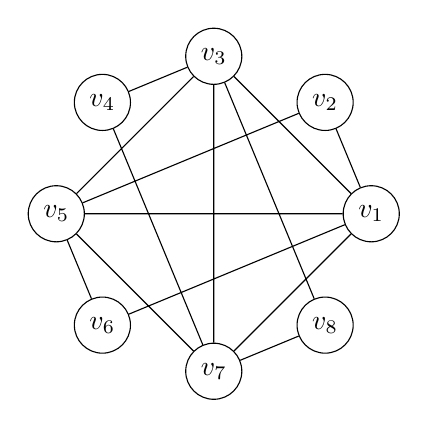
\begin{tikzpicture}[scale=2, bend angle=22.5]
\tikzstyle{every node}=[draw,shape=circle];
\foreach \i in {1,...,8}
{
\path (45*\i-45:1cm) node (v\i) {$v_\i$};
}
\draw
(v1) -- (v2) (v3) -- (v4) (v5) -- (v6) (v7) -- (v8)
(v1) -- (v3) (v3) -- (v5) (v5) -- (v7) (v7) -- (v1)
(v2) -- (v5) (v4) -- (v7) (v6) -- (v1) (v8) -- (v3)
(v1) -- (v5) (v3) -- (v7);
\end{tikzpicture}
\end{center}

Later we will have an introduction to \packagename{tikz} and \packagename{pgf}. If you are interested in it, please refer to the \structure{pgf manual} by \mintinline{shell}|texdoc tikz| or \mintinline{shell}|texdoc pgf|.

\end{frame}

\begin{frame}{Another example}

Binary tree:
\begin{center}
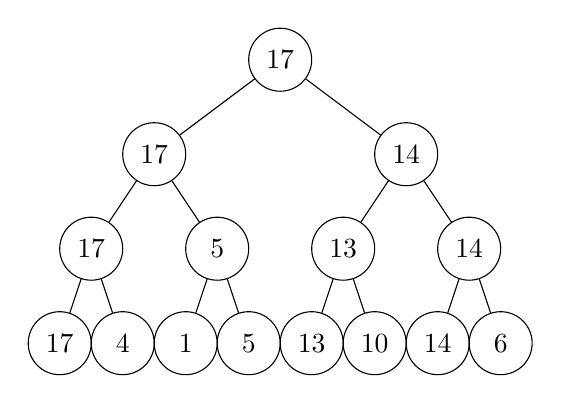
\begin{tikzpicture}[scale=0.8]
\tikzstyle{every node}=[draw,shape=circle,minimum size=0.8cm];
\node {17}[sibling distance=4cm]
child { node {17}[sibling distance=2cm]
	child {
		node {17}[sibling distance=1cm]
		child { node {17} }
		child { node {4} }
	}
	child {
		node {5}[sibling distance=1cm]
		child { node {1} }
		child { node {5} }
	}
}
child { node {14}[sibling distance=2cm]
	child {
		node {13}[sibling distance=1cm]
		child { node {13} }
		child { node {10} }
	}
	child {
		node {14}[sibling distance=1cm]
		child { node {14} }
		child { node {6} }
	}
};
\end{tikzpicture}
\end{center}

\end{frame}

\section{Tables}

\subsection{Tabulars}

\begin{frame}[fragile]{The \packagename{tabular} Environment}
	Table is another common element in \LaTeX, usually you will need the \packagename{booktabs, multirow} packages for enhanced functions of tables. You can insert the command in the preamble of your document.

\begin{command}
\LC|\usepackage{booktabs, multirow}|
\end{command}

\begin{latexexamplesplit}
\begin{tabular}{lcr}
  \toprule
  Title 1 & Title 2 & Title 3 \\
  \midrule
  1 & 2 & 3 \\
  \bottomrule
\end{tabular}
\end{latexexamplesplit}

The syntax is similar to the \packagename{align} environment in maths. \LC|&| is used to split the columns are \LC|\\| is used to split the rows.

\end{frame}

\begin{frame}{Warning}
  \begin{warning}
      Never, ever use vertical lines in tables.
      
      Never use double rules in tables.
  \end{warning}
  \medskip
  They are not professional!
  
  Please read \urllink{http://mirrors.ctan.org/macros/latex/contrib/booktabs/booktabs.pdf} for instructions on designing professional tables.
\end{frame}


\begin{frame}[fragile]{Column Format}

\begin{command}
\begin{LCL}
\begin{tabular}{format}
...
\end{tabular}
\end{LCL}
\end{command}

	\packagename{format} can be set as follow:
	\begin{itemize}
		\item \packagename{|} - vertical line (not recommended)
		\item \packagename{l} - align left in this column
		\item \packagename{c} - align center in this column
		\item \packagename{r} - align right in this column
	\end{itemize}
	\begin{example}
		\begin{minipage}{0.48\linewidth}
			\centering
			\packagename{lll} \medskip
			
        	\begin{tabular}{lll}
        		\toprule
        		Title 1 & Title 2 & Title 3 \\
        		\midrule
        		1 & 2 &3 \\
        		\bottomrule
        	\end{tabular}
		\end{minipage}
		\begin{minipage}{0.48\linewidth}
			\centering
			\packagename{c|cc} \medskip
			
        	\begin{tabular}{c|cc}
        		\toprule
        		Title 1 & Title 2 & Title 3 \\
        		\midrule
        		1 & 2 &3 \\
        		\bottomrule
        	\end{tabular}
		\end{minipage}
    \end{example}	
\end{frame}

\begin{frame}[fragile]{Combining Rows and Columns}

There are two commands being used to combine rows and columns
\begin{command}
\LC|\multicolumn{ncols}{format}{text}|

\begin{itemize}
	\item \packagename{ncols} - the number of columns to be merged
	\item \packagename{format} - the format of the merged column, excluding the left \packagename{|}
	\item \packagename{text} - the text in the merged column
\end{itemize}

\LC|\multirow{nrows}{width}[fixup]{text}|

\begin{itemize}
	\item \packagename{nrows} - the number of rows to be merged
	\item \packagename{width} - the width of the merged rows (use \packagename{*} for auto)
	\item \packagename{fixup} - the vertical position of the text (optional, default in the center)
	\item \packagename{text} - the text in the merged row
\end{itemize}	

\end{command}

To use the \LC|\multirow| command, you need to insert the package \packagename{multirow} in the preamble of your document.

\end{frame}

\begin{frame}[fragile]{Horizontal lines}
  There are four commands to create a horizontal line in a table.

  \begin{itemize}
    \item \LC|\toprule| - Top line
    \item \LC|\midrule| - Middle line
    \item \LC|\cmidrule{2-3}| - Middle line that you can choose the columns to be drawn
    \item \LC|\bottomrule| - Bottom line
  \end{itemize}
  \pause
  \begin{example}
    \begin{minted}{latex}
\begin{tabular}{ccccc}
  \toprule
  \multirow{4}{*}{Table} & Title 1 & Title 2 & Title 3 & Title 4 \\
  \cmidrule{2-5}
  & \multicolumn{2}{c}{Text 1} & 
  \multicolumn{2}{c}{\multirow{3}{*}{Text 3}} \\
  \cmidrule{2-3}
  & \multicolumn{2}{c}{Text 2} & \multicolumn{2}{c}{} \\
  \cmidrule{2-3}
  & Text 4 & Text 5 & \multicolumn{2}{c}{} \\
  \bottomrule
\end{tabular}
    \end{minted}
  \end{example}
\end{frame}

\begin{frame}[fragile]

\begin{latexexample}
\centering
\begin{tabular}{ccccc}
  \toprule
  \multirow{4}{*}{Table} & Title 1 & Title 2 & Title 3 & Title 4 \\
  \cmidrule{2-5}
  & \multicolumn{2}{c}{Text 1} & 
  \multicolumn{2}{c}{\multirow{3}{*}{Text 3}} \\
  \cmidrule{2-3}
  & \multicolumn{2}{c}{Text 2} & \multicolumn{2}{c}{} \\
  \cmidrule{2-3}
  & Text 4 & Text 5 & \multicolumn{2}{c}{} \\
  \bottomrule
\end{tabular}
\end{latexexample}
\medskip
Just leave blank in the rest rows of \LC|\multirow|.

\end{frame}


\begin{frame}[fragile]{Table Generators}
	With \LC|\multirow| and \LC|\multicolumn|, we can almost draw tables of any style, but this coding process can never be as easy as the graphic one, like making tables in Word or Excel. Is there any ways to convert graphic tables into \LaTeX\ codes directly?\\
	\begin{itemize}
		\item Use \LaTeX\ Table Generator: \url{http://www.tablesgenerator.com/}
		\item \LaTeX\ Complex Table Editor: \url{https://www.latex-tables.com/}
		\item Excel2latex: \url{https://ctan.org/tex-archive/support/excel2latex/}
	\end{itemize}
\end{frame}

\subsection{Tables}

\begin{frame}[fragile]{The \packagename{table} Environment}

The \packagename{table} environment is used to arrange the place of a tabular, similar to the \packagename{figure} environment. Here is a template of how to use the environment.

\begin{command}
\begin{LCL}
\begin{table}[position]
  \centering
  \caption{caption}
  \begin{tabular}{format}
    ...
  \end{tabular}
  \label{table:label}
\end{table}
\end{LCL}
\end{command}

The \packagename{position}, \packagename{caption}, \packagename{label} are same as those in the \packagename{figure} environment.
It's recommended to put the caption above the table.
\end{frame}

\begin{frame}[fragile]{Recall the Positions}
	We usually want to place the graphs or tables just below or above the content where we mention them, but even when we type \packagename{[h]} in position, you can not ensure that it will appear at the ideal position, and there are several methods to make up for this. You can try them one by one: \medskip
	\pause
	\begin{enumerate}[<+->]
		\item Change \packagename{[h]} to \packagename{[!h]}
		\item Change \packagename{[!h]} to \packagename{[!H]}
		\item Use \LC|\newpage| to move the following content to the next page
	\end{enumerate}\medskip
	\pause
Usually you don't need to pay too much attention about where the figures and tables are exactly are because you can use \LC|\ref| to reference them. And the numbering of 	figures and tables will strictly follow the order of their code.
	
\end{frame}


\section*{References}

\begin{frame}{References}
    \begin{thebibliography}{9}
        \bibitem{wikibook}
        Wikibook. \url{https://en.wikibooks.org/wiki/LaTeX}.
        \bibitem{overleaf}
        Overleaf Knowledge Base. \url{https://www.overleaf.com/learn}.
        \bibitem{techji}
        linsyking, fakefred et al. \LaTeX\ Lecture. \url{https://github.com/linsyking/latex-wksp}.
        \bibitem{techji}
        tc-imba, zhang et al. \LaTeX\ Lecture. \url{https://github.com/SJTU-UMJI-Tech/LaTeX}.
    \end{thebibliography}
\end{frame}

\begin{frame}{Resources}
    \begin{itemize}
        \item \href{https://wch.github.io/latexsheet/}{\LaTeX\  Cheet Sheet}
        \item \href{https://www.ctan.org/}{The Comprehensive \TeX\ Archive Network}
        \item \href{https://github.com/egeerardyn/awesome-LaTeX}{Awesome \LaTeX}
    \end{itemize}
\end{frame}

\end{document}
